\documentclass[10pt, letterpaper]{article}

% Packages:
\usepackage[
    ignoreheadfoot, % set margins without considering header and footer
    top=1 cm, % seperation between body and page edge from the top
    bottom=0 cm, % seperation between body and page edge from the bottom
    left=2 cm, % seperation between body and page edge from the left
    right=2 cm, % seperation between body and page edge from the right
    footskip=1.0 cm, % seperation between body and footer
     % showframe % for debugging 
]{geometry} % for adjusting page geometry
\usepackage{titlesec} % for customizing section titles
\usepackage{tabularx} % for making tables with fixed width columns
\usepackage{array} % tabularx requires this
\usepackage[dvipsnames]{xcolor} % for coloring text
\definecolor{primaryColor}{RGB}{0, 79, 144} % define primary color
\usepackage{enumitem} % for customizing lists
\usepackage{fontawesome5} % for using icons
\usepackage{amsmath} % for math
\usepackage[
    pdftitle={Kumaravel Rajan's CV},
    pdfauthor={Kumaravel Rajan},
    pdfcreator={LaTeX with RenderCV},
    colorlinks=true,
    urlcolor=primaryColor
]{hyperref} % for links, metadata and bookmarks
\usepackage[pscoord]{eso-pic} % for floating text on the page
\usepackage{calc} % for calculating lengths
\usepackage{bookmark} % for bookmarks
\usepackage{lastpage} % for getting the total number of pages
\usepackage{changepage} % for one column entries (adjustwidth environment)
\usepackage{paracol} % for two and three column entries
\usepackage{ifthen} % for conditional statements
\usepackage{needspace} % for avoiding page brake right after the section title
\usepackage{iftex} % check if engine is pdflatex, xetex or luatex

\usepackage{graphicx}

% Ensure that generate pdf is machine readable/ATS parsable:
\ifPDFTeX
    \input{glyphtounicode}
    \pdfgentounicode=1
    % \usepackage[T1]{fontenc} % this breaks sb2nov
    \usepackage[utf8]{inputenc}
    \usepackage{lmodern}
\fi



% Some settings:
\AtBeginEnvironment{adjustwidth}{\partopsep0pt} % remove space before adjustwidth environment
\pagestyle{empty} % no header or footer
\setcounter{secnumdepth}{0} % no section numbering
\setlength{\parindent}{0pt} % no indentation
\setlength{\topskip}{0pt} % no top skip
\setlength{\columnsep}{0cm} % set column seperation
\makeatletter
\let\ps@customFooterStyle\ps@plain % Copy the plain style to customFooterStyle
% \patchcmd{\ps@customFooterStyle}{\thepage}{
%     \color{gray}\textit{\small Kumaravel Rajan - Page \thepage{} of \pageref*{LastPage}}
% }{}{} % replace number by desired string
\makeatother
\pagestyle{customFooterStyle}

\titleformat{\section}{\needspace{4\baselineskip}\bfseries\large}{}{0pt}{}[\vspace{1pt}\titlerule]

\titlespacing{\section}{
    % left space:
    -1pt
}{
    % top space:
    0.3 cm
}{
    % bottom space:
    0.2 cm
} % section title spacing

\renewcommand\labelitemi{$\circ$} % custom bullet points
\newenvironment{highlights}{
    \begin{itemize}[
        topsep=0.10 cm,
        parsep=0.10 cm,
        partopsep=0pt,
        itemsep=0pt,
        leftmargin=0.4 cm + 10pt
    ]
}{
    \end{itemize}
} % new environment for highlights

\newenvironment{highlightsforbulletentries}{
    \begin{itemize}[
        topsep=0.10 cm,
        parsep=0.10 cm,
        partopsep=0pt,
        itemsep=0pt,
        leftmargin=10pt
    ]
}{
    \end{itemize}
} % new environment for highlights for bullet entries


\newenvironment{onecolentry}{
    \begin{adjustwidth}{
        0.2 cm + 0.00001 cm
    }{
        0.2 cm + 0.00001 cm
    }
}{
    \end{adjustwidth}
} % new environment for one column entries

\newenvironment{twocolentry}[2][]{
    \onecolentry
    \def\secondColumn{#2}
    \setcolumnwidth{\fill, 4.5 cm}
    \begin{paracol}{2}
}{
    \switchcolumn \raggedleft \secondColumn
    \end{paracol}
    \endonecolentry
} % new environment for two column entries

\newenvironment{header}{
    \setlength{\topsep}{0pt}\par\kern\topsep\centering\linespread{1.5}
}{
    \par\kern\topsep
} % new environment for the header

\newcommand{\placelastupdatedtext}{% \placetextbox{<horizontal pos>}{<vertical pos>}{<stuff>}
  \AddToShipoutPictureFG*{% Add <stuff> to current page foreground
    \put(
        \LenToUnit{\paperwidth-2 cm-0.2 cm+0.05cm},
        \LenToUnit{\paperheight-1.0 cm}
    ){\vtop{{\null}\makebox[0pt][c]{
        \small\color{gray}\textit{Last updated in September 2024}\hspace{\widthof{Last updated in September 2024}}
    }}}%
  }%
}%

% save the original href command in a new command:
\let\hrefWithoutArrow\href

% new command for external links:
\renewcommand{\href}[2]{\hrefWithoutArrow{#1}{\ifthenelse{\equal{#2}{}}{ }{#2 }\raisebox{.15ex}{\footnotesize \faExternalLink*}}}

% new command to simplify underline and bold font
\newcommand{\ubf}[1]{\underline{\textbf{#1}}}

\pagenumbering{gobble}

\begin{document}
    \newcommand{\AND}{\unskip
        \cleaders\copy\ANDbox\hskip\wd\ANDbox
        \ignorespaces
    }
    \newsavebox\ANDbox
    \sbox\ANDbox{}

    % \placelastupdatedtext
    \begin{twocolentry}{
        \begin{figure}
        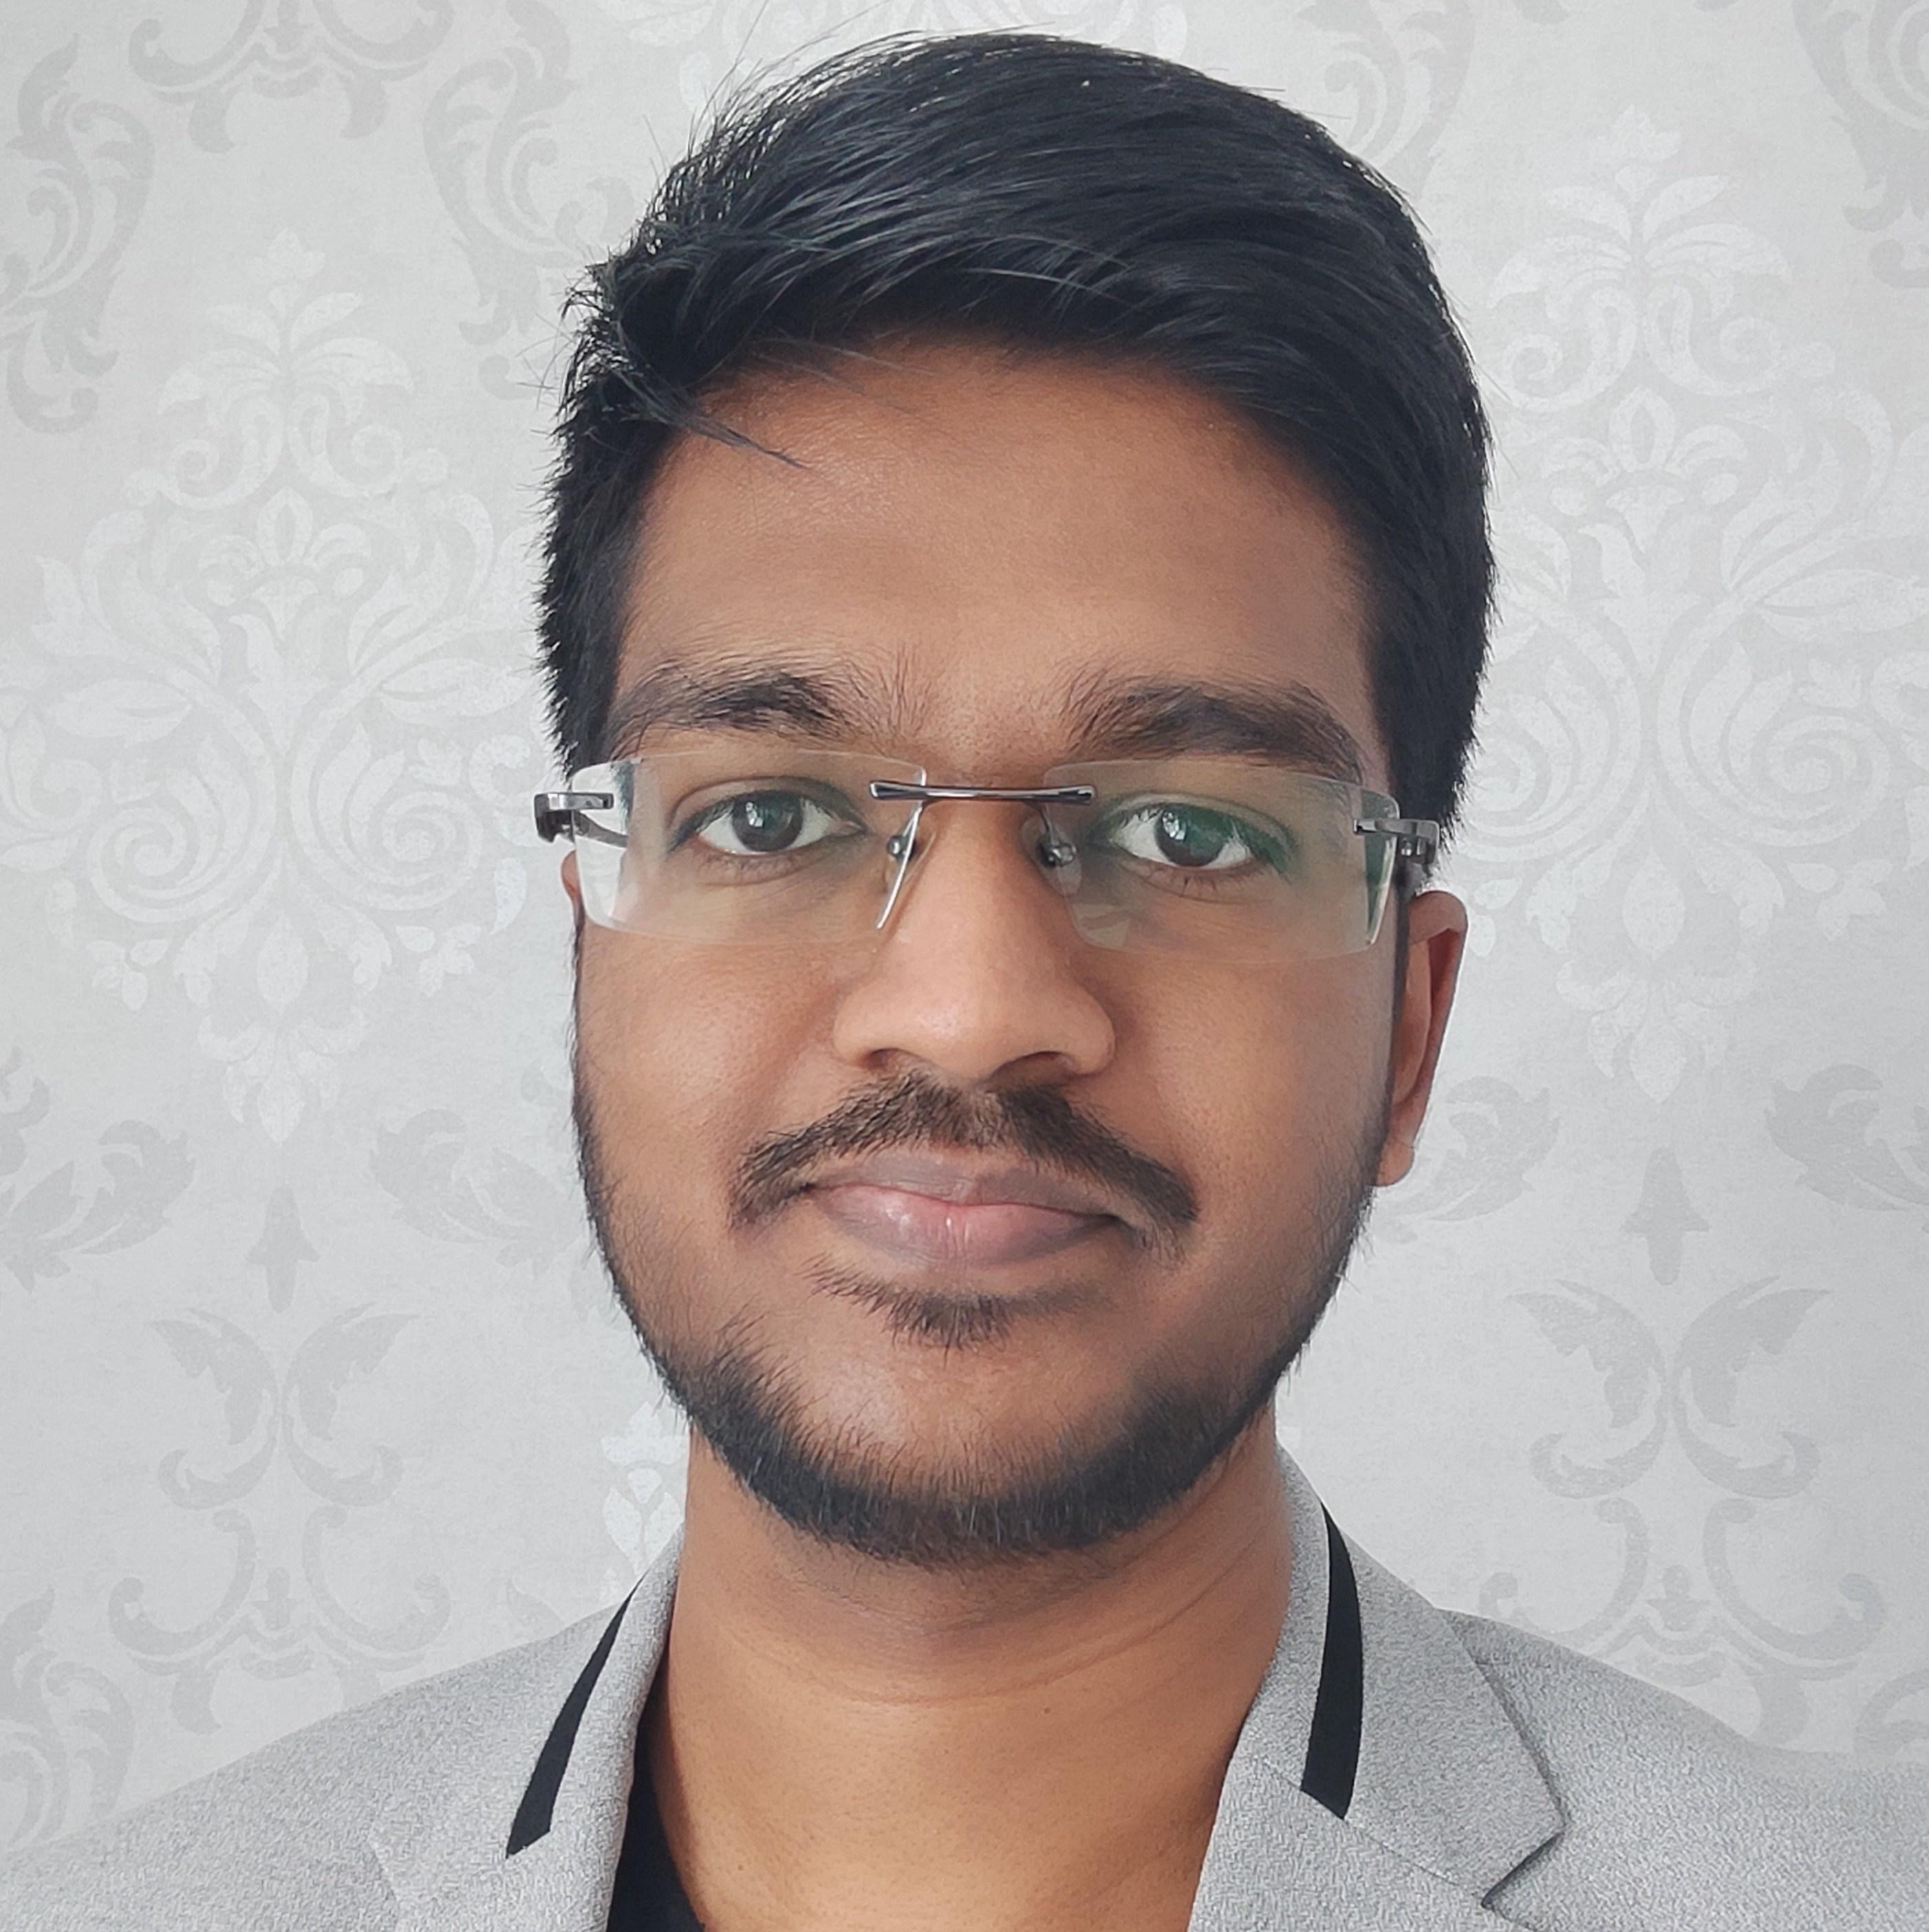
\includegraphics[width=0.17\textwidth]{Kumaravel_latest.jpg}
    \end{figure}
    }
    
    \begin{header}
        \textbf{\fontsize{24 pt}{24 pt}\selectfont Kumaravel Rajan}

        \vspace{0.3 cm}

        \normalsize
        \mbox{Location:\hspace*{0.13cm}Frankfurt}%
        \kern 0.25 cm ;
        \AND%
        \kern 0.25 cm%
        \mbox{\href{mailto:kumaravel.rajan7@gmail.com}{Email:\hspace*{0.13cm}kumaravel.rajan7@gmail.com}}\\%
        \mbox{\href{tel:+4915731143682}{Tel:\hspace*{0.13cm}+49 1573 1143 682}}%
        \kern 0.25 cm ;
        \AND%
        \kern 0.25 cm%
        \mbox{\href{https://www.linkedin.com/in/kumaravel-rajan/}{LinkedIn:\hspace*{0.13cm}kumaravel-rajan}}\\
        \mbox{\href{https://github.com/kumaravelrajan}{Github:\hspace*{0.13cm}kumaravelrajan}}%
        \kern 0.25cm ;
        \AND%
        \kern 0.25 cm%
        \mbox{{Languages:\hspace*{0.13cm}English - C1, German - ca. B2}}%
        \AND%
        \kern 0.25 cm%
        \mbox{{Visa - Chancenkarte (Opportunity card) - Germany}}%
    \end{header}

    \end{twocolentry}

    \vspace{0.3 cm - 0.3 cm}


%####################################################################

    \begin{samepage}

        % \vspace{-0.4 cm}
        

        \section{Education}

        
        \begin{twocolentry}{
            

        \textit{Munich, DE}
            
        \textit{2021 - {2025}}
        
        }
            \textbf{MS in Computer Science}

	    \textit{TU Munich}

            
        \end{twocolentry}

        \vspace{0.10 cm}
        \begin{onecolentry}
            \begin{highlights}
                \item \textbf{Focus}: Software engineering and testing with projects in {data analysis}, web dev, and {distributed systems}.
            \end{highlights}
        \end{onecolentry}

        \end{samepage}

        \vspace{0.2cm}

        % \newpage

        \begin{samepage}

        \begin{twocolentry}{
            

        \textit{Chennai, IN}
            
        \textit{2014 - 2018}
        
        }
            \textbf{BS in Computer Science}

	    \textit{SRM Institute of Science \& Tech}

            
        \end{twocolentry}

        \end{samepage}

%####################################################################

    \section{Relevant Skills}

    % \vspace{0.5cm}



    
    \begin{onecolentry}
        \textbf{Programming Languages:} \ubf{Typescript/Javascript}, {Python}, C++
    \end{onecolentry}

    \vspace{0.2 cm}

    \begin{onecolentry}
        \textbf{Technologies:} 
        \begin{itemize}
            \item \textbf{Software Testing} - \ubf{Jest (JS)}, {unittest (Python)}
            \item \textbf{Web development} - \ubf{{React}, {Node.js}, Express.js}, PostgreSQL, REST API.
            \item \textbf{Version control \& workflows} - {Git}, code reviews
            \item \textbf{Modern development tools} - VScode
            % \item \textbf{Data analysis and visualization}: {Pandas, Matplotlib}.
            \item \textbf{AI coding harness}: \ubf{Opencode}
            % \item \textbf{some prior experience} - Cmake, Qt.
        \end{itemize}
        
    \end{onecolentry}

    % \vspace{0.2cm}

    \section{Experience}
        
        \begin{twocolentry}{
        \textit{Munich, DE}    
            
        \textit{2021 – {2025}}}
            \textbf{Werkstudent Security Analyst}
            
            \textit{Siemens AG}
        \end{twocolentry}

        \vspace{0.10 cm}
        \begin{onecolentry}
            \begin{highlights}
                \item \ubf{Automated data collection by writing {JS web parsers}} with a comprehensive, structured test suite using \ubf{Jest}. Caused a \ubf{27\% uptick in notifications created}.
            \end{highlights}
        \end{onecolentry}


        \vspace{0.3 cm}

        \begin{samepage}
            
        \begin{twocolentry}{
        \textit{Bengaluru, IN}    
            
        \textit{2018 – 2020}}
            \textbf{C++ Software Developer}
            
            \textit{Siemens India}
        \end{twocolentry}

        \vspace{0.10 cm}
        \begin{onecolentry}
            \begin{highlights}
                \item Responsible for system critical bug fixes in a {mature C++ codebase} {for Siemens Comfort HMI Panels}.
                \item \ubf{Introduced TLS} in the previously plaintext communication between Comfort panels and PLCs.
                \item Built an inventory management system using \ubf{React and Node.js along with an interactive dashboard}.
            \end{highlights}
        \end{onecolentry}

        \end{samepage}

	% \vspace{0.2cm}

%#####################################################################

%####################################################################

% \vspace{0.5cm}

\section{Projects}

        \begin{samepage}
             \begin{twocolentry}{ }
            \textbf{Modern Customer support application}

            \textit{Imero GmbH}
            \end{twocolentry}
    
            \vspace{0.10 cm}
            \begin{onecolentry}
                \begin{highlights}
                    \item {Built a {customer support tool} with chat functionality} from scratch using \ubf{Node.js and React} for Imero's support team.
                    \item Tested using \ubf{Jest and Postman}.
                    
                \end{highlights}
            \end{onecolentry}
        \end{samepage}

        \vspace{0.2cm}

        \begin{samepage}
            \begin{twocolentry}{
            \textit{\href{https://github.com/kumaravelrajan/thePegasusEffect.git}{Github}}}
        
            \textbf{The Pegasus Effect}

            \textit{TU Munich}
            \end{twocolentry}

            \vspace{0.10 cm}
            \begin{onecolentry}
            \begin{highlights}
                \item {Collected, cleaned, and analyzed open-source social media data} on Pegasus Spyware victims using Python. Data was analyzed and visualized using {Pandas and Matplotlib}. 
            \end{highlights}
        \end{onecolentry}
        \end{samepage}

        \vspace{0.2cm}

        \begin{samepage}
             \begin{twocolentry}{ \textit{\href{https://github.com/kumaravelrajan/ChordPlusPlus}{Github}}}
            \textbf{ChordPlusPlus}

            \textit{TU Munich}
            \end{twocolentry}
    
            \vspace{0.10 cm}
            \begin{onecolentry}
                \begin{highlights}
                    \item Built a {fault-tolerant, distributed hash table in modern C++}. Tested using \ubf{GTest}.
                \end{highlights}
            \end{onecolentry}
        \end{samepage}

        
        
\end{document}